%%%%%%%%%%%%%%%%%%%%%%%%%%%%%%%%%%%%%%%%%%%%%%%%%%%%%%%%%%%
\section{Theory}
\label{sec:theory}
%%%%%%%%%%%%%%%%%%%%%%%%%%%%%%%%%%%%%%%%%%%%%%%%%%%%%%%%%%%
This section examines the problem of mapping with uniform inputs in 1 and 2 dimensions. For ease of exposition this section represents workspaces as discretised regions. Future work should extend this to continuous regions.
 
\subsection{Mapping in 1D}
We begin with the single particle case, then proceed to the $n$ particle case. 
\subsubsection{1D mapping with 1 particle}
A particle is initialized uniformly randomly in a linear free-space $m$ units wide.  To \emph{map} this region the particle needs to choose one direction, move until it hits a boundary, and then switch direction and move until it reaches the other boundary.


Without loss of generality, assume the particle always starts going left, and label the free-space from 1 to $m$ left to right.  If the initial position is 1, the particle tries to move 1 unit to the left, but is stopped by the boundary. The particle then moves $m-1$ moves to the right.  The final $m^{\textrm{th}}$ move right results in a collision with the right wall, and thus mapping requires $m+1$ moves. This is the minimum number of moves.  The worst case is if the particle starts at $m$, requiring $2m$ moves: $m$ moves to the left and $m$ moves to the right.

The expected number of moves for one particle to cover a 1D area of length $m$ is 
\begin{align}
\frac{1}{m} \sum _{i=1}^m (i+m) &= \frac{3 m+1}{2}  \label{eq:expectedMoves1particle1D}
\end{align}

\subsubsection{1D mapping with n particles}

\begin{figure}
\begin{center}
	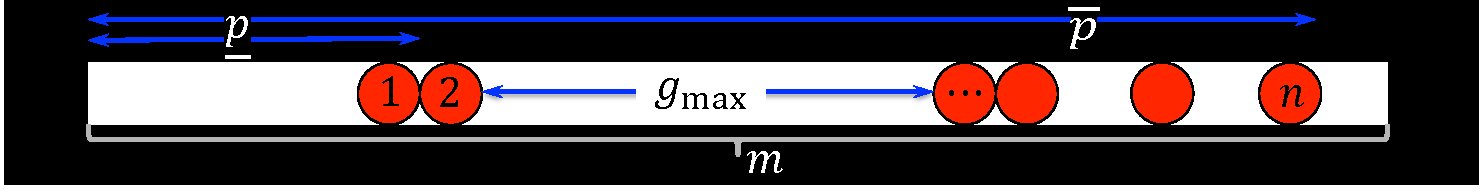
\includegraphics[width=1.0\columnwidth]{MaxGapm20n5s1v3.pdf}
\end{center}
\caption{\label{fig:coverage1d}
Exploring a 1D environment of size $m$ with $n$ particles of unit size. Here $m=20$ and $n=6$. $\pmin=4$, $\pmax=19$ and $g_{max}= 7$
}
\end{figure}

For $n>1$ the average expected number of moves is calculated as follows.
Let $\mathbf{p}$ be the list of positions of $n$ unit size particles uniformly distributed from $[1, m]$.
As shown in Fig. \ref{fig:coverage1d}, the number of moves to discover the left and right boundaries is bounded by the maximum and minimum particles $ \pmin =\min(\mathbf{p})$, $\pmax =\max(\mathbf{p})$, requiring moving left $\pmin$, followed by a move of $m-(\pmax - \pmin )+1 $ right.
When $n=m$, the algorithm requires 2 moves, one left, one right.
The minimum time with $n\in[2,m-1]$ occurs with $\pmin$ at 1 and $\pmax$ at $m$, requiring 3 moves, 1 left followed by 2 moves to the right.  

The maximum $2(m-n+1)$ occurs when the particles are arranged from $m-n$ to $m$, requiring $m-n+1$ moves to the left, followed by $m-n+1$ moves to the right.

This is drawing without replacement $n$ times from the set $[1, m]$.  The minimum is distributed between 1 and $m-n$, the maximum is distributed between $n$ and $m$.

The expected number of moves to reach both boundaries for $n$ particles in 1D is 

\begin{align}
{\scriptstyle \frac{1}{{m \choose n}} \sum_{\pmin = 1}^{m-n+1}  \sum_{\pmax = \pmin +n-1}^{m}   {\pmax -\pmin-1 \choose n-2} \left( 2 \pmin +m- \pmax +1\right)-\frac{\left(m-n+1\right)}{{m \choose n}}} \nonumber
\\= \frac{3(1+m)}{1+n} - \frac{\left(m-n+1\right)}{{m \choose n}}
\label{eq:expectedMoveskparticles1D}
 \end{align}

This reduces to Eqn.~\eqref{eq:expectedMoves1particle1D} when $n=1$. To fully map the area from 1 to $m$ requires that every position from 1 to $m$ be visited by at least one particle. This time is dominated by the maximum gap $\overline{g}$. The total number of moves is then $ 2 \pmin +m- \pmax +1 + \max \left( \overline{g} - \left(\pmin + m-\pmax \right),0 \right)$.


 Since these particles are unit size, there are $m-n$ spaces, and these can be located before, between, or after the $n$ particles in $n+1$ locations giving ${m-n \choose n+1}$ possible configurations. The largest gap can be calculated exactly using a recurrence equation \cite{reviriego2011expected}, but a tight bound when
$m>n \log{n}$ is $\frac{m-n}{n+1} + \Theta \left( \sqrt{\frac{ (m-n)\log(n+1)}{n+1}} \right)$\cite{Raab1998}. 

%\todo{I want an analytical result for the expected maximum gap. An analytical result for the maximum gap is given in \url{http://www.nebrija.es/~jmaestro/esa/papers/JDA2011.pdf}, but I have been unable to solve the coefficients in equation (18).  The same result is also in Section 9.4 of An Introduction to the Analysis of Algorithms, Second Edition by Robert Sedgewick and Philippe Flajolet, which I have ordered but don't have yet. -Aaron}
%Define the probability of any given combination $T= {m \choose n}^{-1}$.  
%If $n+1 = m$ there is one gap of size $1$, and $n+1$ possible locations.
%The maximum gap size is $m-n$, and this gap can be placed before or after any of the $n$  numbers, for a total of $n+1$ possible positions.


\subsubsection{1D mapping with scan and move costs}
 Often scanning (imaging) and moving the particles costs time and energy.
 When controlling particles with MRI as in \cite{chanu2008adapting}, the MRI machine iterates between imaging and applying gradient forces to move the particles.
 This section examines 1D mapping when scanning the workspace and moving the particles a unit distance have associated costs. 
The objective is to minimize a linear combination of costs for moving and measuring; however, the precise respective coefficients may be subject
to change, or even unknown in advance turning this into a {\em bicriteria problem}, in which both parameters need to be within 
a bounded ratio of those in an optimal solution. For simpler notation, we write $(a,b)$ for a schedule that involves $a$ unit steps and $b$ scans.

For a more detailed analysis, assume that the left boundary is located $D$ units to the left of the leftmost particle.
(This analysis can be applied in both directions.)
The theoretically optimal, yet elusive, solution requires scanning the workspace to map particle locations,
moving $D+1$ units to the left, 
then scanning to detect that the leftmost particle has only moved $D$ units and thus has encountered the wall,
for a total cost of $(D+1,2)$ for the schedule.

We can achieve a schedule with $D+1$ steps by scanning after each step, for a total cost of $(D+1,D+2)$;
while this is optimal with respect to steps, the involved scan cost is large compared to the optimum.
At the expense of increasing the number of steps we can reduce the number of scans by successively doubling the number 
of steps between scans, i.e., performing the $i^{\textrm{th}}$ scan after $2^i$ steps, resulting in total cost at most $(2D+2,\log_2 D)$; replacing
the base of $2$ by an arbitrary constant $k$, we get $(k\times(D+1), \log_k D)$. This is within a constant of the optimal. 
On the other hand, moving a sufficiently large number $M$ of steps (known to satisfy $M\geq D$) before performing the second 
scan yields $(M,2)$, which is optimal with respect to scan cost, but bad in terms of the cost for motion.

Balancing the competitive factor for both parameters can be achieved as follows:
perform the $i$th scan at position $i^i$. This yields a simultaneous competitive factor of $O(\log D/\log\log D)$ for {\em both} parameters.

\begin{theorem}
\label{th:eyetoeye}
The hyperexponential search sequence $i^i$ yields a best possible simultaneous competitive factor of $O(\log D/\log\log D)$ for {\em both} parameters
of the bicriteria search problem.
\end{theorem}

\begin{proof}
Let us first consider the number of scans.
If the boundary is properly detected in step $j+1$, the particle must have encountered it between steps $j$ and $j+1$, i.e. $j^j \leq D < (j+1)^{j+1}$.
Now we can employ the Lambert $W$ function, which is the inverse function of $f(x)=xe^x$; note that 
$$\log x = W(\log x) \cdot e^{W(\log x)},$$ 
so
	$$\log \log x = (\log W(\log x) + W(\log x)),$$
and therefore
	$$W(\log x) \in \Theta(\log \log x).$$

This implies that $j\leq \log D/ W(\log D)$ (the inverse of $j^j$), hence $\Theta(\log D/ \log\log D)+1$ scans have been made, while the optimum are $2$ scans.

The moved distance is $(j+1)^{j+1}$, while the optimum is $D\geq j^j$.
Hence, we get the ratio 
\begin{align}
\frac{(j+1)^{(j+1)}}{j^j}=(j+1)\frac{(j+1)^j}{j^j},\label{eq:MoveDistanceRatio}
\end{align}
 where $0\leq \frac{(j+1)^j}{j^j}\leq \mathrm{e}$ for $j>0$.
 
Because $j\leq \log D/ W(\log D)$, we obtain 
\begin{align}
\frac{(j+1)^{(j+1)}}{j^j}\leq \mathrm{e}\frac{\log n}{ W(\log n)}+\mathrm{e}\label{eq:MoveDistanceRatioInequality}
\end{align}
 for $j>0$. Clearly, this is again in within a factor of $\Theta(\log D/ \log\log D)$ of the optimum.
 
 To see that this balanced factor is best possible, observe that $\left(\frac{\log D}{\log\log D}\right)^{\left(\frac{\log D}{\log\log D}\right)}\in \Theta(D)$, with the base corresponding to the ratio between step lengths and the exponent to the number of scans. Therefore, using significantly fewer than $\log D/ \log\log D$ scans would require increasing the base, yielding a worse competitive factor for the step length; on the other hand, decreasing the base in order to decrease the competitive factor for the step length would require increasing the exponent, yielding a worse competitive factor for the scan cost.
\end{proof}

%\subsubsection{German tank problem}
%With multiple samples it is now possible to guess which direction is closer to the edge?  The population maximum is 
%uniformly minimum-variance unbiased estimator "The sample maximum plus the average gap between observations in the sample" --> but this will give the same distance to each side.  

\subsection{Mapping in 2D}


\subsubsection{2D mapping with 1 particle}
The shortest path for mapping with 1 particle is a version of depth-first search that halts when all frontier cells have been explored.
As long as the all the free cells are connected, depth-first-search (DFS) is the optimal solution to mapping.
%\todo{Q2.Domink --- Prove that DFS is the optimal solution with 1 particle }
%<Dominik> <- this tag is just to ease possible merges. Feel free to edit or delete.
Even if the environment is known in advance, the problem is NP-hard as can be shown by a trivial reduction to Hamiltonian paths in grid graphs \cite{itai1982hamilton}. %NP-hardness shown in Itai, Alon, Christos H. Papadimitriou, and Jayme Luiz Szwarcfiter. "Hamilton paths in grid graphs." SIAM Journal on Computing 11.4 (1982): 676-686.
One can easily show that a simple DFS guarantees a competitive ratio of $2$: the depth-first tree has $m-1$ edges and each edge is traversed at most twice. 
Any path that covers $m$ cells needs to traverse least $m-1$ edges, and hence the depth-first-search is at most twice as long as an optimal coverage path.

For showing that no algorithm can perform better one needs only a simple 1-dimensional graph that goes to the left and to the right.
If the algorithm chooses to go arbitrarily to one side, we can make it do a long walk of length $m$ and then return it just for a single field on the other side ($2m+1$ vs.\ $2+m$).
If the algorithm decides to switch the direction after some time after arbitrary zig-zags (of increasing cost) of cost $z$ (center to one side to other side) we decide that there is a single field on both sides.
The algorithm now needs to go one additional time from one side to the other and back (cost $>z$) while the optimum cost would have been $\leq z+3$.
If the algorithm switches from the second form to the first, the first argument still applies.

%TOURS (related work, actually doesn't belong here but you probably find it here most easily. Just to help with related work.):
Most previous work on grid graph exploration focused on exploration tours, i.e., after exploration one has to go back to the start position.
If the environment is known in advance, this equals the traveling salesman problem and a polynomial-time approximation scheme is known~\cite{klein2008linear}. % Philip N. Klein.  A linear-time approximation scheme for TSP in undirected  planar  graphs  with  edge-weights.  SIAM  Journal  on  Computing , 37(6):1926–1952, 2008.
If the environment is unknown, as it is in our case, the best achievable competitive ratio is $2$ in general grid graphs (achieved by depth first search) and $7/6$ for simple grid graphs ($4/3$ achieved by smartDFS \cite{icking2005exploring}). %Icking et al. http://link.springer.com/chapter/10.1007/11533719_53 http://www.geometrylab.de/applet-55
%</Dominik>

\subsubsection{2D mapping with $n$ particles}

Another problem with this type of mapping is identifying which move sequence guarantees the shortest path in the worst case.
%At the beginning there can be at most four frontier cells per particle to be explored. 
 %As the particles begin to move, the number of frontier cells explored and the number of free cells identified increases. 
 
 We describe three algorithms of increasing complexity for 2D mapping.
 If we implement a random move algorithm as described in {\sc RandomMoves}, at each step the particles all move in the same randomly selected direction until there are no frontier cells left on the map. 
 \emph{MoveType} is a vector that holds the four possible move types. 
 The map $\mathbf{M}$ is a matrix the size of the work space. 
 Each cell of  $\mathbf{M}$ holds one of five values that denote: \emph{Particle}, \emph{Frontier}, \emph{Unknown}, \emph{Freespace} and \emph{Obstacle}. 
 At each step {\sc Frontier} returns the locations of frontier cells in $\mathbf{M}$ and $\mathbf{r}$ has the list of particle locations.
 The \emph{move} is implemented to update the map $\mathbf{M}$ and the particle locations $\mathbf{r}$ by calling {\sc Move\&\!Update}. 
{\sc RandomMoves} requires minimal computation and is probabilistically complete, so eventually the swarm maps the free cells~\cite{kahn1989cover}. 
 However, this method of mapping is inefficient, resulting in long mapping times, especially with small numbers of particles in large, torturous maps with many turns. 

  \begin{algorithm}
\caption{\sc RandomMoves($\mathbf{M},\mathbf{r}$)   \label{alg:randommove}}
\begin{algorithmic}[1]
\State \emph{MoveType}$ = \{l,r,u,d\}$ 
\While{$|${\sc Frontier}$(\mathbf{M})| >0  $}
%\While{ $|\mathbf{M}.Frontiercells| >0  $}
\State \emph{move} $ \gets$ {\sc random}$($\emph{MoveType}$)$
\State $\{\mathbf{M}, \mathbf{r}\} \gets ${\sc Move\&\!Update}$(move, \mathbf{M}, \mathbf{r}) $
\EndWhile
\end{algorithmic}
\end{algorithm}

A better way to map the world is to deliberately move particles toward frontier cells. 
We could choose one particle as the $elect$ particle and perform motion planning using this particle. 
In {\sc ElectParticle}, one of the particles is selected as \emph{elect}. 
As long as the number of frontiers to be visited is at least one, the algorithm proceeds by generating a $mvSq$ from the current position of the elect particle to the nearest frontier cell. 
The \emph{mvSq} is generated by a breadth-first-search (BFS) shortest path algorithm which requires the map $\mathbf{M}$, source \emph{elect}, and the cells {\sc Frontier}$(\mathbf{M})$. A representative $mvSq$ is $\langle u,r,d,d,r,u,\ldots\rangle$. 
The list of moves in \emph{mvSq} are implemented by iteratively calling the {\sc Move\&\!Update} function for the length of $mvSq$. 


{\sc ElectParticle} will explore the target frontier cell by the end of $mvSq$. 
However, often with large-population swarms the whole $mvSq$ need not be implemented. 
Every time {\sc Move\&\!Update} is called, the nearest frontier is updated and $mvSq$ is also updated because as the particles start to move, the target frontier cell  might be explored by a non-elect  particle. 

 {\sc ClosestFrontier} exploits this fact by computing a BFS shortest path from all particles to all frontier cells.   
  \begin{algorithm}
\caption{\sc ElectParticle($\mathbf{M},\mathbf{r}$)   \label{alg:ElectParticle}}
\begin{algorithmic}[1] 
\State \emph{elect} $ \gets$ {\sc random}$(\mathbf{r})$
\While{$|${\sc Frontier}$(\mathbf{M})| >0  $}
\State \emph{mvSq} $ \gets$ BFS$(\mathbf{M},$\emph{elect}$,${\sc Frontier}$(\mathbf{M}))$
\For { \emph{iter} $:=1$ $\mathbf{ to}$ $|$\emph{mvSq}$| $ $\mathbf{ step }$ $ 1$} 
\State $\{\mathbf{M}, $\emph{elect}$\} \gets ${\sc Move\&\!Update}$($\emph{mvSq}$, \mathbf{M}, $\emph{elect}$) $
 \EndFor
\EndWhile
\end{algorithmic}
\end{algorithm}

In each loop of {\sc ClosestFrontier}, all the moves in $mvSq$ are implemented to explore the target frontier cell since it is the shortest possible route to a frontier cell. 
At time 0, there will be at most 4$n$ equally valid destinations that can be visited since cells to the side of each particle not neighboring another particle are frontier cells. 
%Our BFS expands the search in order, ${l,r,u,d}$, so the first move is $l$. 
Each $mvSq$ guarantees classification of one frontier cell into obstacle or free space.
When a frontier cell is explored it is labeled either free or obstacle. There can be a net gain of at most two frontier cells per particle that encounters a free cell or no new frontier cells if the frontier cell contained an obstacle. 

 
The simulation results in Section \ref{sec:simulation} show that both map complexity and distribution affect the number of moves taken to map the work space. {\sc RandomMove} uses no information from the data except for checking completion. {\sc ElectParticle} uses the location and distance data from one particle to map the work space. {\sc ClosestFrontier} improves the performance of mapping by using all the data. 

  \begin{algorithm}
\caption{\sc ClosestFrontier($\mathbf{M},\mathbf{r}$) \label{alg:ClosestFrontier}}
\begin{algorithmic}[1]
\While{$|${\sc Frontier}$(\mathbf{M})| >0  $}
\State$mvSq \gets$ BFS$(\mathbf{M},\mathbf{r},${\sc Frontier}$(\mathbf{M}))$
\For {$iter:=1$ $\mathbf{ to}$ $|mvSq| $ $\mathbf{ step }$ $ 1$}  
\State $\{\mathbf{M},\mathbf{r}\} \gets ${\sc Move\&\!Update}$(mvSq, \mathbf{M}, \mathbf{r}) $

 \EndFor
  
\EndWhile
\end{algorithmic}
\end{algorithm}
%<Dominik>
 %Comment: Just some quick text because this section is still missing. Feel free to remove or change.
While {\sc ClosestFrontier} is usually the more reasonable approach in practice than DFS with a single particle, we are only able to show a trivial weaker bound on the corresponding moves. {\sc ClosestFrontier} is not optimal. It can need $\Omega(n^2)$ moves while an optimal strategy only needs $O(n)$.
An example can be seen in Fig.~\ref{fig:square-worse-than-opt}.
In some scenarios {\sc ClosestFrontier} can perform worse than DFS with a single particle, e.g., in Fig.~\ref{fig:greed-worse-than-dfs}.



\begin{figure}
\begin{center}
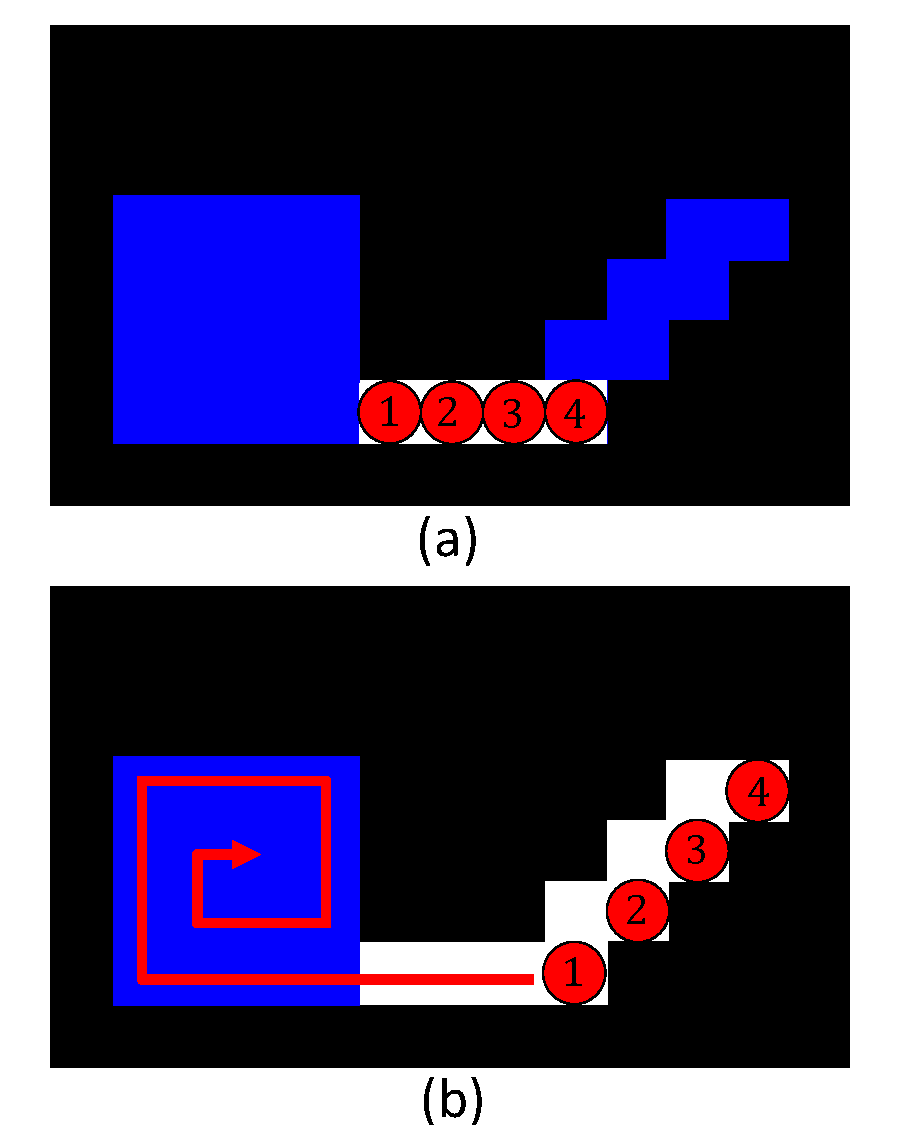
\includegraphics[width=1.0\columnwidth]{greedy2}
\end{center}
\caption{\label{fig:square-worse-than-opt}
{\sc ClosestFrontier} is not optimal in all cases. {\sc ClosestFrontier}, which is greedy, could go right first and then cover the square with a single particle which takes $\Omega(n^2)$ moves while the optimal solution, which visits the square in parallel using all $n$ particles, only needs $O(n)$ moves.}
\end{figure}
	
\begin{figure}
\begin{center}	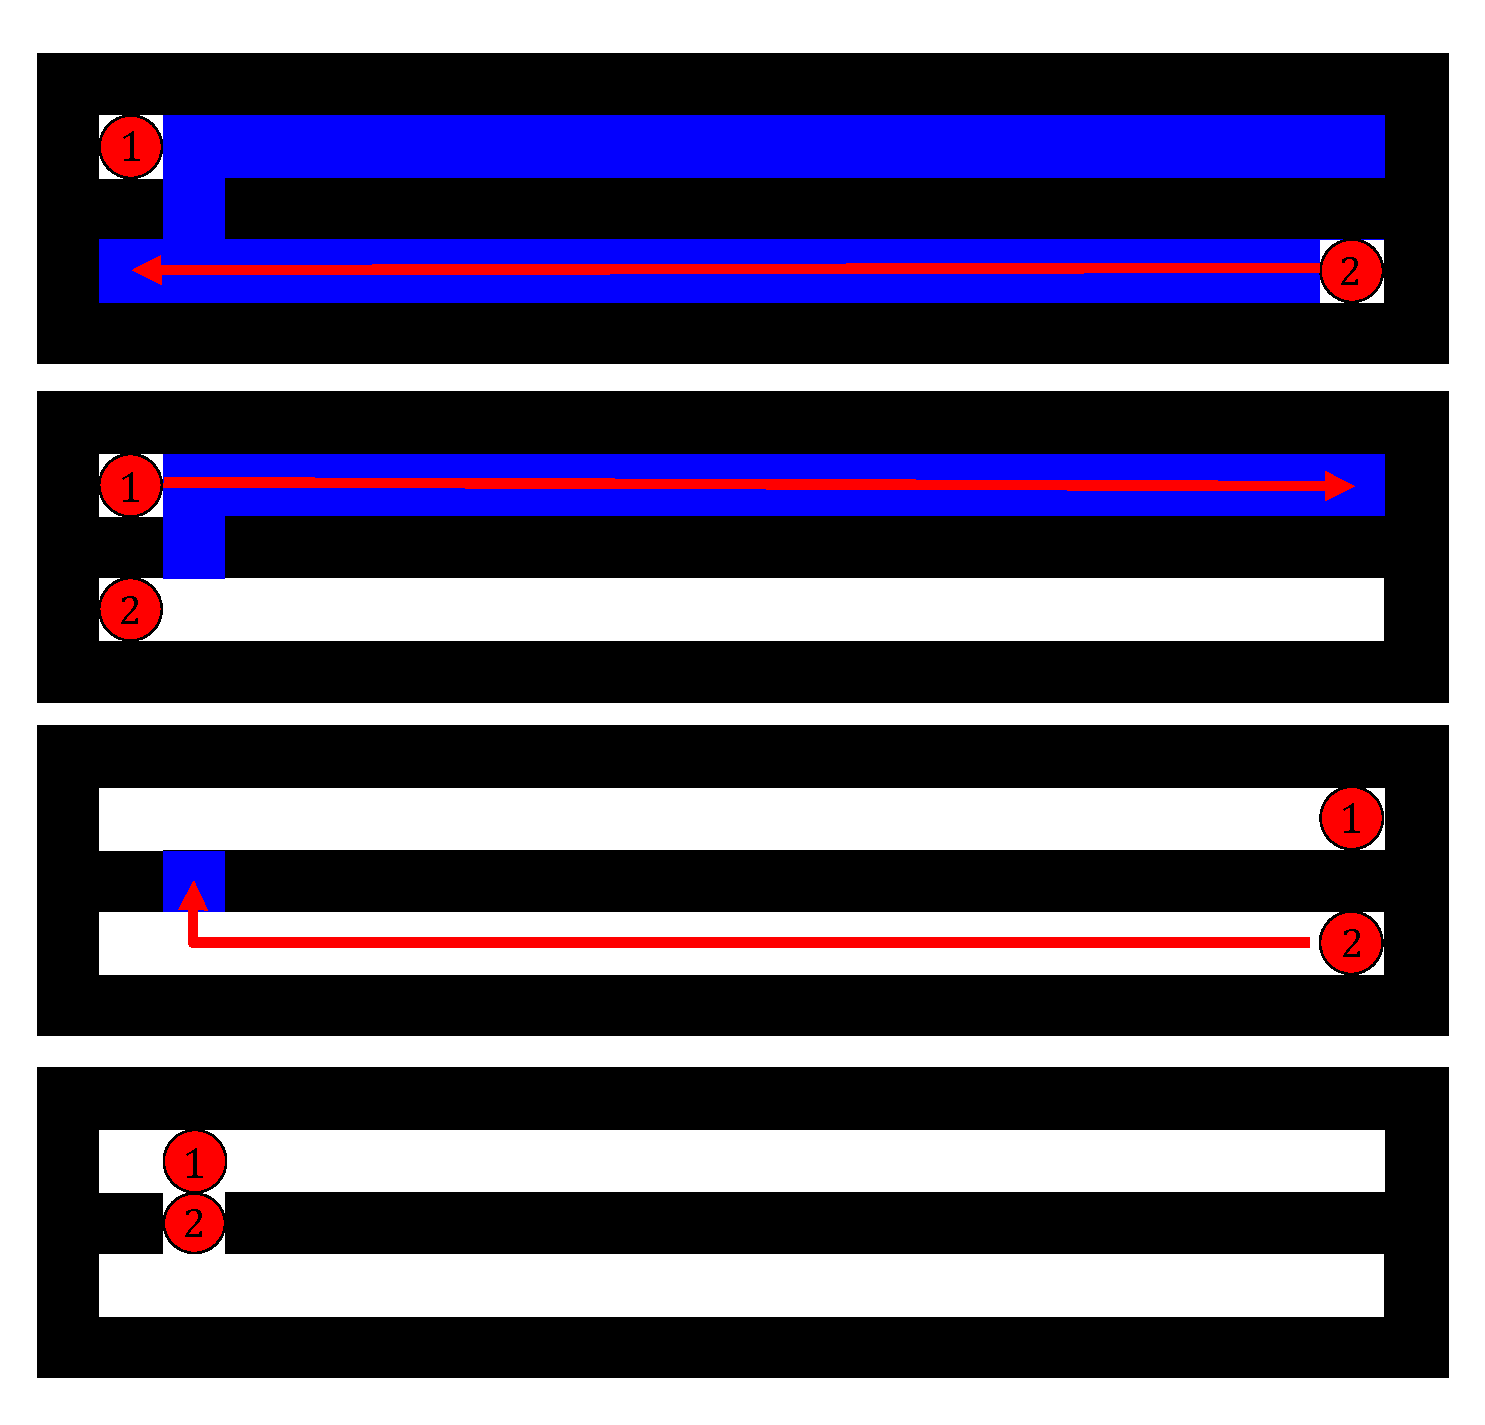
\includegraphics[width=0.8\columnwidth]{greedy1}
\end{center}
\caption{\label{fig:greed-worse-than-dfs}
{\sc ClosestFrontier} can be worse than DFS in some cases as well. In this example, using {\sc ClosestFrontier} is $1.5\times$ worse than DFS using only particle 2.}
%If the move preference order is $\{l,u,r,d\}$ using Alg.~\ref{alg:ClosestFrontier}. then coverage with two particles takes approximately 1.5 times longer than with just the bottom right particle.
\end{figure}

%\begin{figure}
%	\centering
%	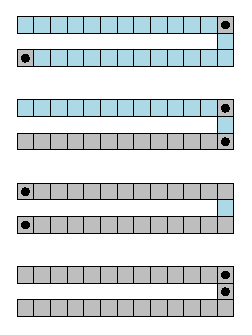
\includegraphics[width=0.2\textwidth]{greedy-worse-than-dfs.eps}
%	\caption{In this example, the greedy strategy is $1.5\times$ worse than DFS with the bottom left particle.}
%	\label{fig:greed-worse-than-dfs}
%\end{figure}
%TRIVIAL UPPER BOUND
\begin{theorem}
	{\sc ClosestFrontier} needs at most $O(m^2)$ moves where $m$ is the number of cells. 
\end{theorem}
\begin{proof}
	The distance between a particle and the closest frontier cell can be at most the number of all already visited cells.
	Hence, the distance for visiting the $i^{\textrm{th}}$ field is bounded by $i$.
	The overall number of moves is bounded by $\sum_{i=1,\ldots,m} i = 0.5\cdot m\cdot (m+1)$.
\end{proof}
%</Dominik>

%\todo{insert plot of boundary nodes as a function of moves for 3 different values of no. of particles. n=100, n=500 and n=2000} 



%Better if particles are in a square with side $\sqrt{N}$ and are in a vertical column spaced $\sqrt{N}/k-1$ apart.  moving left, followed by moving
%<Dominik>
%Comment: Just some quick text because this section is still missing. Feel free to remove or change.


%\begin{figure}
%	\centering
%	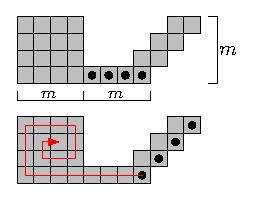
\includegraphics[width=0.2\textwidth]{square-bad-case.eps}
%	\caption{If the move preference is counter clockwise, the greedy strategy might selects to go right and then covers the square with a single particle which takes $\Omega(m^2)$ moves while the optimal strategy that visits the square in parallel with the $m$ particles, only needs $O(m)$ moves.}
%	\label{fig:square-worse-than-opt}
%\end{figure}
%</Dominik>

%\todo{Q4.What is the complexity of the 2D problem? 
%NP-hard already for 1-particle, see previous section. The decision problem is NP-complete (i.e., it's not worse than NP-hard). %Dominik
%}

%\todo{Q5.Can we do better than the greedy algorithm for 2D coverage?  }

%\todo{Q6.What is the running time for the greedy algorithm?  }
%<Dominik>
%Comment: Just some quick text because this section is still missing. Feel free to remove or change.
\begin{theorem}
	{\sc ClosestFrontier} has a computational complexity in $O(m^2)$.
\end{theorem}
\begin{proof}
	For an environment with $m$ cells, there are at most $m$ iterations.
	Since the edges in the grid graph are not weighted and each cell only has at most four neighbors, the shortest path from a particle to the frontier cell can be calculated in $O(m)$ time by a simple breadth first search.
	%NOTE: CURRENTLY USING DIJKSTRA WHICH HAS A HIGHER COMPLEXITY.
\end{proof}
%</Dominik>

%Completion time is a function of the initial particle distribution. The minimum mapping time for a rectangle $n$ units tall and $m/n$ wide, with the $n$ particles arranged along the left wall. 1 move left registers the left wall, repeating $m/n$ moves up, down, and right to find the top and bottom boundaries and move right until reaching the right boundary.  This requires $3(m/n)+1$ moves. %1+2(N/K) + 2(N/k -1)+1 = 

%Better if particles are in a square with side $\sqrt{N}$ and are in a vertical column spaced $\sqrt{N}/k-1$ apart.  moving left, followed by moving
Finally, completion time is also a function of the map geometry.
Mapping requires exploring all the free spaces and the boundary of the free spaces.
The number of map cells that need to be explored is the \emph{Area} $+$ \emph{Perimeter} $-~n$. 
This is minimized by a circular region and maximized by a linear region.
 For example,  a linear region has $m+(2m+2)-n$ cells to explore, while a 
 square region has $m + (4 \sqrt{m}) -n$ cells to explore.

%a $5\times4$ rectangular grid, then the number of map cells that need to be classified is only $a\cdot b+2(a+b)-n=33$ where $a=5$ and $b=4$.  
%  Fig.~\ref{fig:greedy1} shows a scenario where two particles perform worse than one particle. 
 % Here for $m$=43, it takes the two particles 60 moves to complete coverage whereas if particle 2 alone is present, it would take 44 moves. 
 % This shows that particle distribution is key to determining the number of moves taken. This behavior is also seen in the simulation experiment in Sec.~\ref{sec:simulation}. 
%  But in general, for a uniform random spread of particles the algorithm works better on an average with a small standard deviation.





%\subsection{Mapping in 3D}

%\todo{We can do some experiments for this.  Perhaps draw wireframes for free spaces, draw red and blue cubes for unknown.  TODO: draw with red circles/spheres for particles.}





